\usubsection{Incremento 2: Ejecución distribuida y soporte para recursividad}

El segundo incremento se planteó con el propósito de expandir el alcance del sistema desde la ejecución local hacia un modelo distribuido. A partir de la evaluación del incremento anterior, se identificaron como necesidades principales la integración de hardware externo, específicamente tarjetas micro:bit, la ejecución de subflujos en computadoras remotas y la incorporación de mecanismos que permitieran resolver la limitación detectada con respecto a la recursividad.

El trabajo del incremento se organizó en cuatro líneas de desarrollo:

\begin{itemize}
    \item Diseño e implementación de un protocolo de comunicación con tarjetas micro:bit.
    \item Construcción de un servidor orquestador para la distribución de tareas entre múltiples computadoras mediante WebSockets.
    \item Ampliación del catálogo de nodos con componentes de control de hardware, interacción con el usuario y lógica condicional avanzada.
    \item Implementación de soporte para recursividad en el paradigma de flujos de datos.
\end{itemize}

Se planificó además la verificación de compatibilidad de los protocolos de comunicación en los principales navegadores web.

Para habilitar la ejecución de lógica en el hardware educativo, se diseñó un protocolo denominado \emph{Micro:bit Dataflow Protocol~1.0} (DFP1). Se estableció un canal de comunicación que soporta tanto USB Serial (Web Serial en navegadores) como BLE UART (Web Bluetooth en navegadores), los principales canales de comunicación remota disponibles en las tarjetas micro:bit~V2. Dado que el enlace Bluetooth posee una unidad máxima de transferencia (MTU) limitada, a menudo truncando mensajes cercanos a los 20~caracteres, se diseñó un mecanismo de fragmentación. Los mensajes se estructuran como líneas de texto terminadas en salto de línea, manteniendo una longitud controlada para evitar pérdidas de datos.

Se definió que los subflujos creados en el editor visual se compilarían a un formato binario personalizado denominado DFBC1 (\emph{Dataflow Byte Code~1.0}). Este formato incluye un encabezado con metadatos y una sección de instrucciones basada en una máquina de pila LIFO (\emph{Last-In, First-Out}). El motor en el micro:bit procesaría comandos específicos (como \texttt{ADD}, \texttt{CONCAT} y \texttt{RETURN}) que consumen operandos de la pila, ejecutan la operación y devuelven el resultado. El proceso de comunicación se dividió en fases de transmisión de metadatos (\texttt{BEGIN}), envío del bytecode fragmentado (\texttt{CHUNK}) y confirmación del programa (\texttt{COMMIT}). Una vez que el programa reside totalmente en la memoria del micro:bit, el orquestador envía un comando de ejecución (\texttt{RUN}) con los argumentos necesarios y recibe posteriormente los resultados o eventos de vuelta en el navegador a través del canal establecido. La especificación detallada de este protocolo se encuentra en el Apéndice~\ref{apx:microbit-protocol}.

Para la distribución de tareas entre múltiples computadoras, se modeló una arquitectura cliente-servidor basada en WebSockets, tecnología seleccionada por su capacidad de mantener canales bidireccionales persistentes y de baja latencia, esenciales para la sincronización de un flujo de datos en tiempo real. Se definió un servidor central que actuaría como orquestador del sistema, cuya responsabilidad principal sería gestionar el ciclo de vida del grafo de ejecución global. Al iniciar el programa, el orquestador analizaría el flujo y determinaría qué nodos debían ejecutarse localmente y cuáles debían delegarse a otros dispositivos conectados (denominados internamente \emph{workers}). Se diseñó una tabla de estado de las conexiones de modo que, al recibir un resultado parcial de una PC remota, el orquestador actualizaría las dependencias de los nodos subsiguientes y, al cumplirse las condiciones de disparo, enviaría inmediatamente las nuevas instrucciones al dispositivo correspondiente o las ejecutaría localmente según el caso. Este diseño centralizado simplifica la gestión de la concurrencia y asegura que los datos fluyan correctamente entre dispositivos heterogéneos. En la Figura~\ref{fig:orchestrator-incr2} se muestra un esquema de la arquitectura modelada.

\begin{figure}[H]
    \centering
    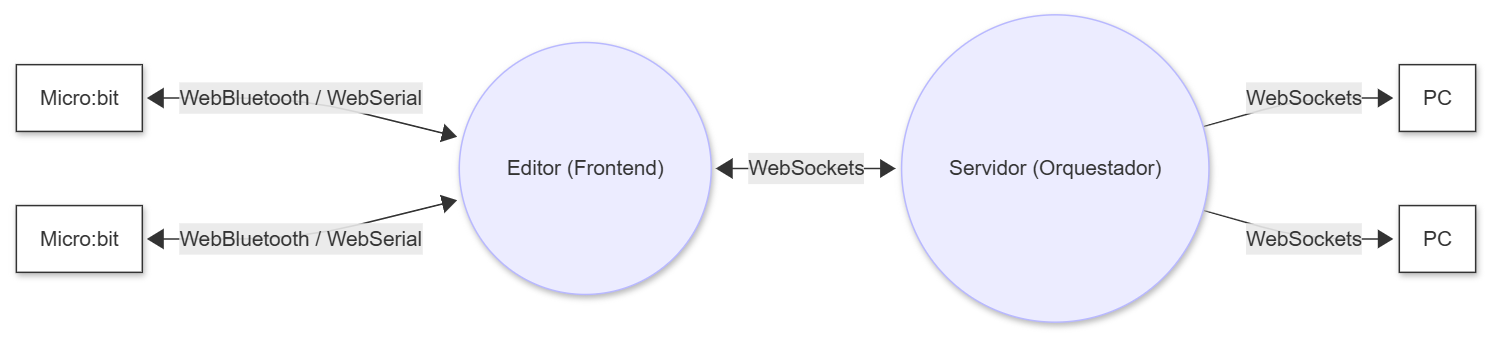
\includegraphics[width=\textwidth]{../images/ws-orchestrator-architecture.png}
    \caption[Esquema de comunicación distribuida]{\normalfont Esquema de comunicación distribuida entre el orquestador y los dispositivos}
    \label{fig:orchestrator-incr2}
\end{figure}

Para el soporte de recursividad, se diseñó un mecanismo basado en el nodo de abstracción de subflujos. El estudiante podría instanciar dicho nodo dentro de su propio lienzo interno, haciendo explícita la autorreferencia y asumiendo la responsabilidad de construir los casos base. El control se estructuró en dos fases. Durante la inicialización del motor, un contexto global rastrearía las plantillas de subflujo activas, reutilizando la definición ya registrada al detectar una llamada recursiva en lugar de repetir el análisis, lo que evita ciclos de resolución infinitos. En tiempo de ejecución, un contexto dinámico actuaría como una pila de llamadas controlada, donde cada invocación generaría una instancia independiente del motor de ejecución para aislar los datos.

La construcción siguió los diseños descritos. Se implementó el protocolo DFP1 con su compilador de subflujos a DFBC1, el mecanismo de fragmentación de mensajes para ambos canales (serial y Bluetooth) y el servidor orquestador con la tabla de estado de conexiones y la distribución dinámica de tareas hacia los \emph{workers}.

La implementación del soporte para recursividad incorporó, además de lo previsto en el modelado, un contador de profundidad por cada cadena de invocaciones: si el caso base del estudiante falla y se alcanza un límite máximo de seguridad preestablecido, el sistema intercepta el flujo y detiene la ejecución con una excepción, garantizando un equilibrio entre la libertad del usuario y la protección del entorno en el navegador. Esta limitación se hizo considerando su impacto sobre la completitud de Turing del lenguaje, que, aunque no permite la iteración ilimitada, sigue siendo capaz de expresar una amplia gama de algoritmos recursivos comunes en la enseñanza de programación, como el cálculo de factoriales o la generación de secuencias de Fibonacci; lo que se considera suficiente para el alcance del proyecto.

Para soportar las nuevas capacidades distribuidas y ampliar las funcionalidades del lenguaje, se incorporaron los siguientes nodos al catálogo:

\begin{itemize}
    \item \textbf{Control de micro:bit.} Nodos específicos para interacciones puntuales con las tarjetas, tales como Leer botón, Escribir en matriz LED y Emitir sonido, que permiten la comunicación directa con el hardware.
    \item \textbf{Interacción con el usuario.} Nodos de Leer (solicitud de datos por teclado) y Opción Aleatoria, para la generación de datos desde el entorno local.
    \item \textbf{Lógica de control.} El nodo \emph{Condicional + Selector}, que evalúa condiciones lógicas y dirige el flujo de datos hacia una de diferentes salidas. Este nodo representó una evolución sobre el planteamiento original, que se basaba en el enrutamiento a través de un \emph{switch}: el nuevo enfoque permite mayor flexibilidad e independencia entre los datos usados en las condiciones y los datos de salida para cada caso.
    \item \textbf{Editor de fórmulas.} Un nodo especializado que permite redactar expresiones matemáticas mediante una sintaxis textual simplificada, en lugar de una interconexión extensiva de nodos aritméticos básicos. El componente actúa como evaluador de expresiones en tiempo de ejecución, procesando múltiples variables de entrada y consolidando el cálculo en una única salida. Esta adición facilita la transición de los jóvenes hacia formas de pensamiento más abstractas y simbólicas.
\end{itemize}

La validación del segundo incremento se centró en comprobar la viabilidad técnica de la ejecución en hardware externo y computadoras remotas. Se realizaron pruebas de comunicación entre el navegador y dispositivos micro:bit a través de Web Serial y Web Bluetooth, así como pruebas de orquestación entre múltiples computadoras conectadas por WebSockets. Se verificó el envío y reconstrucción correcta de programas fragmentados, la ejecución remota de subflujos y la recepción de resultados en el entorno principal. También se validó el soporte para recursividad mediante subflujos con autorreferencia y casos base definidos por el usuario.

Dado el uso de múltiples protocolos (Serial, Bluetooth y WebSockets), fue importante validar la compatibilidad entre navegadores. Las pruebas realizadas en Chrome, Firefox, Edge y Safari revelaron que todos los protocolos son soportados por los navegadores basados en Chromium (Chrome y Edge), mientras que Firefox y Safari carecen de soporte para Web Serial y Web Bluetooth. Se consideró suficiente este nivel de compatibilidad, en línea con otras herramientas de programación visual para computación física, como MakeCode y MBlock, que también recomiendan navegadores basados en Chromium para la interacción con micro:bit. El resumen de esta revisión se presenta en la Tabla~\ref{tab:browser-compatibility}.

La evaluación mediante casos de prueba arrojó dos hallazgos significativos. En primer lugar, aunque la infraestructura base soportaba la comunicación y ejecución distribuida, el lenguaje visual carecía de primitivas que facilitaran la orquestación intuitiva de tareas sobre listas. Se identificó la necesidad de implementar nodos de iteración con mayor nivel de abstracción, específicamente constructos inspirados en las operaciones colectivas de MPI, tales como \textit{scatter} y \textit{gather}, para simplificar visualmente los patrones de división de carga y recolección de resultados.

En segundo lugar, se observó que el esquema de integración de las tarjetas micro:bit estaba restringido a un rol pasivo como dispositivos de procesamiento de datos enviados desde el programa principal. Esta limitación reducía la utilidad práctica del lenguaje para modelar aplicaciones orientadas, por ejemplo, al IoT, donde es fundamental la lectura dinámica de sensores. Se planteó, por tanto, la necesidad de implementar un modelo de integración más flexible que permita a los micro:bit actuar como fuentes de datos activas, capaces de emitir información al programa principal en respuesta a cambios en sus sensores, habilitando así la creación de proyectos interactivos y reactivos.

Como resultado de esta iteración, se obtuvo un entorno capaz de ejecutar algoritmos distribuidos donde una parte del procesamiento ocurre en el navegador, otra en dispositivos micro:bit y otra en PCs remotas, todo coordinado de forma transparente por el servidor orquestador. Esta arquitectura validó la viabilidad de la propuesta para soportar sistemas distribuidos de manera accesible para niños y jóvenes. En particular, la integración de la placa micro:bit como nodo de procesamiento autónomo se alinea con los hallazgos de \citeA{espejo2022}, quienes reportan que el uso de agentes tangibles facilita la comprensión de la ejecución concurrente en poblaciones jóvenes.